% 109-15(인쇄 109쪽) — 힌트의 정규분포곡선: 대칭축 x=m(점선)과 양쪽 꼬리 P(X≤6), P(X≥10) 을 색칠한 그림.
% 스캔 화질이 낮아 TikZ 로 다시 그림. 라벨은 원문에 있는 것만(6, m, 10, x) · 구하는 m 의 값은 그림에 적지 않는다.
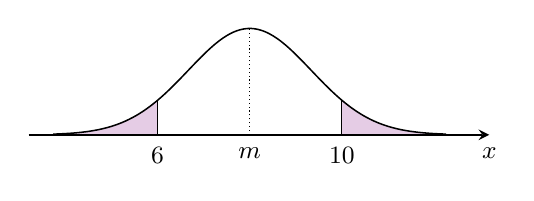
\begin{tikzpicture}[x=0.78cm, y=1.35cm, line width=0.55pt, font=\small]
  \fill[violet!20] plot[domain=-3.2:-1.5, samples=50, smooth] ({\x},{exp(-\x*\x/2)}) -- (-1.5,0) -- (-3.2,0) -- cycle;
  \fill[violet!20] plot[domain=1.5:3.2, samples=50, smooth] ({\x},{exp(-\x*\x/2)}) -- (3.2,0) -- (1.5,0) -- cycle;
  \draw[->, >=stealth, line width=0.7pt] (-3.6,0) -- (3.9,0) node[below=1pt] {$x$};
  \draw plot[domain=-3.2:3.2, samples=110, smooth] ({\x},{exp(-\x*\x/2)});
  \draw[line width=0.4pt] (-1.5,0) -- (-1.5,{exp(-1.125)});
  \draw[line width=0.4pt] (1.5,0) -- (1.5,{exp(-1.125)});
  \draw[densely dotted, line width=0.4pt] (0,0) -- (0,1);
  \node[below=1pt] at (-1.5,0) {$6$};
  \node[below=1pt] at (0,0) {$m$};
  \node[below=1pt] at (1.5,0) {$10$};
\end{tikzpicture}
